\documentclass[a4paper]{article}
\usepackage{geometry}
\usepackage{graphicx}
\usepackage{natbib}
\usepackage{amsmath}
\usepackage{amssymb}
\usepackage{amsthm}
\usepackage{paralist}
\usepackage{epstopdf}
\usepackage{tabularx}
\usepackage{longtable}
\usepackage{multirow}
\usepackage{multicol}
\usepackage[hidelinks]{hyperref}
\usepackage{fancyvrb}
\usepackage{algorithm}
\usepackage{algorithmic}
\usepackage{float}
\usepackage{paralist}
\usepackage[svgname]{xcolor}
\usepackage{enumerate}
\usepackage{array}
\usepackage{times}
\usepackage{url}
\usepackage{fancyhdr}
\usepackage{comment}
\usepackage{environ}
\usepackage{times}
\usepackage{textcomp}
\usepackage{caption}
\usepackage{multirow}


\urlstyle{rm}

\setlength\parindent{0pt} % Removes all indentation from paragraphs
\theoremstyle{definition}
\newtheorem{definition}{Definition}[]
\newtheorem{conjecture}{Conjecture}[]
\newtheorem{example}{Example}[]
\newtheorem{theorem}{Theorem}[]
\newtheorem{lemma}{Lemma}
\newtheorem{proposition}{Proposition}
\newtheorem{corollary}{Corollary}


\floatname{algorithm}{Procedure}
\renewcommand{\algorithmicrequire}{\textbf{Input:}}
\renewcommand{\algorithmicensure}{\textbf{Output:}}
\newcommand{\abs}[1]{\lvert#1\rvert}
\newcommand{\norm}[1]{\lVert#1\rVert}
\newcommand{\RR}{\mathbb{R}}
\newcommand{\CC}{\mathbb{C}}
\newcommand{\Nat}{\mathbb{N}}
\newcommand{\br}[1]{\{#1\}}
\DeclareMathOperator*{\argmin}{arg\,min}
\DeclareMathOperator*{\argmax}{arg\,max}
\renewcommand{\qedsymbol}{$\blacksquare$}

\definecolor{dkgreen}{rgb}{0,0.6,0}
\definecolor{gray}{rgb}{0.5,0.5,0.5}
\definecolor{mauve}{rgb}{0.58,0,0.82}

\newcommand{\Var}{\mathrm{Var}}
\newcommand{\Cov}{\mathrm{Cov}}

\newcommand{\vc}[1]{\boldsymbol{#1}}
\newcommand{\xv}{\vc{x}}
\newcommand{\Sigmav}{\vc{\Sigma}}
\newcommand{\alphav}{\vc{\alpha}}
\newcommand{\muv}{\vc{\mu}}

\newcommand{\red}[1]{\textcolor{red}{#1}}

\def\x{\mathbf x}
\def\y{\mathbf y}
\def\w{\mathbf w}
\def\v{\mathbf v}
\def\E{\mathbb E}
\def\V{\mathbb V}

% TO SHOW SOLUTIONS, include following (else comment out):
\newenvironment{soln}{
    \leavevmode\color{blue}\ignorespaces
}{}


\hypersetup{
%    colorlinks,
    linkcolor={red!50!black},
    citecolor={blue!50!black},
    urlcolor={blue!80!black}
}

\geometry{
  top=1in,            % <-- you want to adjust this
  inner=1in,
  outer=1in,
  bottom=1in,
  headheight=3em,       % <-- and this
  headsep=2em,          % <-- and this
  footskip=3em,
}


\pagestyle{fancyplain}
\lhead{\fancyplain{}{Homework 3}}
\rhead{\fancyplain{}{CS 760 Machine Learning}}
\cfoot{\thepage}

\title{\textsc{Homework 3}} % Title

%%% NOTE:  Replace 'NAME HERE' etc., and delete any "\red{}" wrappers (so it won't show up as red)

\author{
\red{GURUPRASAD VISWANATHAN RAMESH} \\
\red{9082378762}\\
} 

\date{}

\begin{document}

\maketitle 


\textbf{Instructions:} 
Use this latex file as a template to develop your homework. Submit your homework on time as a single pdf file to Canvas. Late submissions may not be accepted. Please wrap your code and upload to a public GitHub repo, then attach the link below the instructions so that we can access it. You can choose any programming language (i.e. python, R, or MATLAB). Please check Piazza for updates about the homework.
\red{Github Link: https://github.com/Guruprasad68/CS760-Machine-Learrning-Spring2023}\\
\red{Code can be found in the ipynb folder of the repo}
\section{Questions (50 pts)}
\begin{enumerate}
\item (9 pts) Explain whether each scenario is a classification or regression problem. And, provide the number of data points ($n$) and the number of features ($p$).\\
\begin{soln}
    The type of our output space decides whether it is a classification or regression problem. In the case of classification, prediction is discrete, and for regression, the output is continuous. 
\end{soln}
\begin{enumerate}
	\item (3 pts) We collect a set of data on the top 500 firms in the US. For each firm we record profit, number of employees, industry and the CEO salary. We are interested in predicting CEO salary with given factors.
	
	\begin{soln}  Since salary is a continuous value, this problem is regression. And $n=500$, $p=3$ \end{soln}
	
	\item (3 pts) We are considering launching a new product and wish to know whether it will be a success or a failure. We collect data on 20 similar products that were previously launched. For each product we have recorded whether it was a success or failure, price charged for the product, marketing budget, competition price, and ten other variables.
	
	\begin{soln}  This is a classification problem as the output is discrete. It can either be a success or a failure. Here, $n=20$. $p=13$  \end{soln}
	
	\item (3 pts) We are interesting in predicting the \% change in the US dollar in relation to the weekly changes in the world stock markets. Hence we collect weekly data for all of 2012. For each week we record the \% change in the dollar, the \% change in the US market, the \% change in the British market, and the \% change in the German market.
	
	\begin{soln} Since \% change is a continuous variable, our problem is regression. Here, $n$ is the number of weeks in a year, i.e., 52, and $p$ equals 3.  \end{soln}
	
\end{enumerate}

\item (6 pts) The table below provides a training data set containing six observations, three predictors, and one qualitative response variable.

\begin{center}
	\begin{tabular}{ c  c  c  c}
		\hline
		$X_{1}$ & $X_{2}$ & $X_{3}$ & $Y$ \\ \hline
		0 & 3 & 0 & Red \\
		2 & 0 & 0 & Red \\
		0 & 1 & 3 & Red \\
		0 & 1 & 2 & Green \\
		-1 & 0 & 1 & Green \\
		1 & 1 & 1 & Red  \\
		\hline
	\end{tabular}
\end{center}

Suppose we wish to use this data set to make a prediction for $Y$ when $X_{1} = X_{2} = X_{3} = 0$ using K-nearest neighbors.

\begin{enumerate}
	\item (2 pts) Compute the Euclidean distance between each observation and the test point, $X_{1} = X_{2} = X_{3}=0$.
 
	\begin{soln}  The euclidean distance of two points $(x_1,y_1,z_1)$ and $(x_2,y_2,z_2)$ is given by: $$\sqrt{(x_1-x_2)^2 + (y_1-y_2)^2 + (z_1-z_2)^2}$$
    Using this formula, we can compute the distance of $(0,0,0)$ from each of the six points in the dataset. The distances are tabulated in the table below: 
    \begin{table}[hbt!]
    \centering
    \begin{tabular}{ccccc}
    \hline
    $X_{1}$ & $X_{2}$ & $X_{3}$ & $Y$ & Distance to (0,0,0) \\ \hline
    0 & 3 & 0 & Red & 3 \\
    2 & 0 & 0 & Red & 2 \\
    0 & 1 & 3 & Red & $\sqrt{10}=3.16$ \\
    0 & 1 & 2 & Green & $\sqrt{5}=2.23$ \\
    -1 & 0 & 1 & Green & $\sqrt{2}=1.41$ \\
    1 & 1 & 1 & Red & $\sqrt{3}=1.73$ \\ \hline
    \end{tabular}
    \end{table}
    
    
    \end{soln}
 
	\item (2 pts) What is our prediction with $K=1$? Why?
	
	\begin{soln}  If $K=1$, then we take the closest point to $(0,0,0)$ and use the label of that point as the prediction of $(0,0,0)$. In this case, the closest point is $(-1,0,1)$ with a distance of 1.414. Thus, the prediction is Green. \end{soln}
	
	\item (2 pts) What is our prediction with $K=3$? Why?
	
	\begin{soln}  If $K=3$, then we'll consider the three closest points to $(0,0,0)$ and use the majority label of the three points as the prediction for $(0,0,0)$. In this case, the three closest points to $(0,0,0)$ are $(-1,0,1)$, $(1,1,1)$, $(2,0,0)$ with distances 1.414, 1.73 and 2 respectively. The majority label of these three is Red, and thus, our prediction of $(0,0,0)$ is Red.\end{soln}

\end{enumerate}

\item (12 pts) When the number of features $p$ is large, there tends to be a deterioration in the performance of KNN and other local approaches that perform prediction using only observations that are near the test observation for which a prediction must be made. This phenomenon is known as the curse of dimensionality, and it ties into the fact that non-parametric approaches often perform poorly when $p$ is large.

\begin{enumerate}
	\item (2pts) Suppose that we have a set of observations, each with measurements on $p=1$ feature, $X$. We assume that $X$ is uniformly (evenly) distributed on [0, 1]. Associated with each observation is a response value. Suppose that we wish to predict a test observation’s response using only observations that are within 10\% of the range of $X$ closest to that test observation. For instance, in order to predict the response for a test observation with $X=0.6$, we will use observations in the range [0.55, 0.65]. On average, what fraction of the available observations will we use to make the prediction?
	
	\begin{soln}  We know that: $ P(a \leq x \leq b) = \int_a^b f(x) dx$, where $f(x)$ is the probability density function of our distribution. In the case of uniform distribution, the pdf is $\frac{1}{b-a}$ and, in our case, $f(x)=1$. Therefore, the integral is equal to $b-a$. Since, we are considering points lying within $10\%$ of $x$, $a=x-0.05$ and $b=x+0.05$. Thus, $ P(x-0.05 \leq x \leq x+0.05)=0.1$. Therefore, on average we can say we will be using 10\% of the available observations to make our prediction. 
    \end{soln}
	
	
	\item (2pts) Now suppose that we have a set of observations, each with measurements on $p =2$ features, $X1$ and $X2$. We assume that predict a test observation’s response using only observations that $(X1,X2)$ are uniformly distributed on [0, 1] × [0, 1]. We wish to are within 10\% of the range of $X1$ and within 10\% of the range of $X2$ closest to that test observation. For instance, in order to predict the response for a test observation with $X1 =0.6$ and $X2 =0.35$, we will use observations in the range [0.55, 0.65] for $X1$ and in the range [0.3, 0.4] for $X2$. On average, what fraction of the available observations will we use to make the prediction?
	
	\begin{soln}  Using the same logic as (a), we can say fraction of available observations within 10\% of $X1$ is 10\%, and  10\% of $X2$ is 10\%. However, the region common to $X1$ and $X2$ is what we're interested in. The probability of a point lying in this region is 0.01 or 1\% of available points in the data on average will be needed for making a prediction.\end{soln}
	
	\item (2pts) Now suppose that we have a set of observations on $p = 100$ features. Again the observations are uniformly distributed on each feature, and again each feature ranges in value from 0 to 1. We wish to predict a test observation’s response using observations within the 10\% of each feature’s range that is closest to that test observation. What fraction of the available observations will we use to make the prediction?
	
	\begin{soln}  Extrapolating the logic of (a) and (b), we get $0.1^{100}$ as the probability of a point lying in the common region of the 10\% range of the 100 features. That is, only $(0.1)^{98}$\% of available observations will be used to make a prediction. This is a very, very small number and would require a huge amount of observations in order to find a single point in the 10\% region. \end{soln}
	
	\item (3pts) Using your answers to parts (a)–(c), argue that a drawback of KNN when p is large is that there are very few training observations “near” any given test observation.
	
	\begin{soln}  Observations in (a)-(c) show empirical evidence for the curse of dimensionality. The probability of finding an observation for a given point reduces as the number of features increases, from what we notice in (a)-(c). The empirical evidence is done using a uniform distribution, and thus a more formal proof that is applicable across all distributions would be a better way to say KNN doesn't do well for high-dimensional data. Also, we are restricting ourselves to 10\% range of each feature instead of K-closest observations for a given point. This  assumption is also crucial in our evidence \end{soln}
	
	\item (3pts) Now suppose that we wish to make a prediction for a test observation by creating a $p$-dimensional hypercube centered around the test observation that contains, on average, 10\% of the training observations. For $p =$1, 2, and 100, what is the length of each side of the hypercube? Comment on your answer.
	
	\begin{soln}  From (a) to (c), we can say that probability of the region we are choosing to find observations for a given point is equal to $a^p$, where a is the side of the hypercube and p is the number of features. Given hypercube volume is 0.1 or 10\%. Thus, we can say: \\
    When p=1, a=0.1\\
    When p=2, $a=0.1^{1/2}$\\
    When p=100, $a=0.1^{1/100}$
    \end{soln}
	
\end{enumerate}

\item (6 pts) Supoose you trained a classifier for a spam detection system. The prediction result on the test set is summarized in the following table.
\begin{center}
	\begin{tabular}{l l | l l}
		&          & \multicolumn{2}{l}{Predicted class} \\
		&          & Spam           & not Spam           \\
		\hline
		\multirow{2}{*}{Actual class} & Spam     & 8              & 2                  \\
		& not Spam & 16             & 974               
	\end{tabular}
\end{center}

Calculate
\begin{enumerate}
	\item (2 pts) Accuracy
	\begin{soln}  Accuracy=$\frac{TP+TN}{TP+FN+TN+FP}=\frac{8+974}{1000}$=0.982 \end{soln}
	\item (2 pts) Precision
	\begin{soln}  Precision=$\frac{TP}{TP+FP}=\frac{8}{24}$=0.33 \end{soln}
	\item (2 pts) Recall
	\begin{soln}  Recall=$\frac{TP}{TP+FN}=\frac{8}{10}$=0.80 \end{soln}
\end{enumerate}


\item (9pts) Again, suppose you trained a classifier for a spam filter. The prediction result on the test set is summarized in the following table. Here, "+" represents spam, and "-" means not spam.

\begin{center}
\begin{tabular}{ c  c }
\hline
Confidence positive & Correct class \\ \hline
0.95 & + \\
0.85 & + \\
0.8 & - \\
0.7 & + \\
0.55 & + \\
0.45 & - \\
0.4 & + \\
0.3 & + \\
0.2 & - \\
0.1 & - \\
\hline
\end{tabular}
\end{center}

\begin{enumerate}
	\item (6pts) Draw a ROC curve based on the above table.
	
	\begin{soln}  For plotting the ROC curve, we need to estimate the True Positive Rate (TPR) and False Positive Rate (FPR). They are defined by: TPR=$\frac{TP}{TP+FN}$ and FPR=$\frac{FP}{TN+FP}$. Using this and considering the points where the actual label changed from + to - as thresholds, we can arrive at Table \ref{tab:roc_ques5}. Using the TPR and FPR values, we can plot the ROC curve, refer to figure \ref{fig:q15a}. \newpage
    \begin{table}[hbt!]
    \centering
    \begin{tabular}{ccc}
    \hline
    Threshold & TPR & FPR \\ \hline
    0.95 &  &  \\
    0.85 & 2/6 & 0 \\
    0.8 &  &  \\
    0.7 &  &  \\
    0.55 & 4/6 & 0.25 \\
    0.45 &  &  \\
    0.4 &  &  \\
    0.3 & 1 & 0.5 \\
    0.2 &  &  \\
    0.1 & 1 & 1 \\ \hline
    \end{tabular}
    \caption{Question 1-5(a): TPR and FPR for various thresholds} \label{tab:roc_ques5}
    \end{table}

    
    \begin{figure}
        \centering
        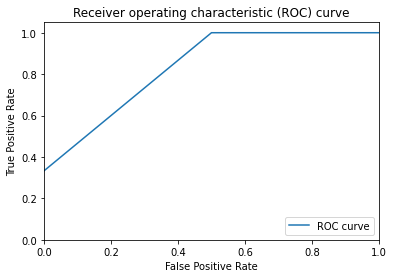
\includegraphics[width=0.4\textwidth, height=50mm]{images/q1_5a_roc.png}
        \caption{ROC Curve obtained from the TPR and FPR values in Table \ref{tab:roc_ques5}}
        \label{fig:q15a}
    \end{figure}
    
    \end{soln}


	\item (3pts) (Real-world open question) Suppose you want to choose a threshold parameter so that mails with confidence positives above the threshold can be classified as spam. Which value will you choose? Justify your answer based on the ROC curve.
	
	\begin{soln}  The application plays a huge role in deciding which threshold we choose for our model. For a spam classifier, it is important for the model to classify spam accurately but not completely at the cost of misclassifying a lot of proper mail. So, a fair point of threshold is 0.55 where TPR=4/6 and FPR=0.25. One could also go for threshold=0.3 if the main goal is to classify spam correctly, where TPR=1, and FPR=0.5. \end{soln}
\end{enumerate}

\item (8 pts) In this problem, we will walk through a single step of the gradient descent algorithm for logistic regression. As a reminder,
$$f(x;\theta) = \sigma(\theta^\top x)$$
$$\text{Cross entropy loss } L(\hat{y}, y) = -[y \log  \hat{y} + (1-y)\log(1-\hat{y})]$$
$$\text{The single update step } \theta^{t+1} = \theta^{t} - \eta \nabla_{\theta} L(f(x;\theta), y) $$



\begin{enumerate}
	\item (4 pts) Compute the first gradient $\nabla_{\theta} L(f(x;\theta), y)$.
	
	\begin{soln}  To compute the gradient, we need to use the chain rule. If $\hat{y}=\sigma(\theta^\top x)=\sigma(z)$. Then,\\
        $$\nabla_{\theta} L(f(x;\theta), y)=\nabla_{\hat{y}} L(f(x;\theta), y)\nabla_{\theta} \hat{y}=\nabla_{\hat{y}} L(f(x;\theta), y)\nabla_{z} \hat{y}\nabla_{\theta} z$$
        Let us proceed by computing each of these terms separately.
        $$\nabla_{\hat{y}} L(f(x;\theta), y)=-[\frac{y}{\hat{y}}-\frac{1-y}{1-\hat{y}}]=-[\frac{y(1-\hat{y})-\hat{y}(1-y)}{\hat{y}(1-\hat{y})}]$$
        $$\nabla_{z} \hat{y}=\sigma(z)(1-\sigma(z))=\hat{y}(1-\hat{y})$$
        $$\nabla_{\theta} z=x$$.\\ \\

        Therefore, multiplying the individual terms we get, $$\nabla_{\theta} L(f(x;\theta), y)=-x[y(1-\hat{y})-\hat{y}(1-y)]=x(\hat{y}-y)$$.
    \end{soln}
	
	\item (4 pts)
 Now assume a two dimensional input. After including a bias parameter for the first dimension, we will have $\theta\in\mathbb{R}^3$.
$$ \text{Initial parameters : }  \theta^{0}=[0, 0, 0]$$
$$ \text{Learning rate }\eta=0.1$$
$$ \text{data example : } x=[1, 3, 2], y=1$$
Compute the updated parameter vector $\theta^{1}$ from the single update step.
	
	\begin{soln}  $\hat{y}=\sigma(\theta^{0\top} x)=\sigma([0,0,0] [1,3,2]^\top)=\sigma(0)=0.5$.\\
    Substituting $\hat{y}$ and the gradient from (a), we have, $\theta^1=\theta^0 - \eta \nabla_{\hat{y}} L(f(x;\theta), y)=[0,0,0]-0.1*[1,3,2](-0.5)=[0.05,0.15,0.1]$.
    $$\theta^1=[0.05,0.15,0.1]$$
 \end{soln}
\end{enumerate}
\end{enumerate}

\section{Programming (50 pts)}
\begin{enumerate}
	\item (10 pts) Use the whole D2z.txt as training set.  Use Euclidean distance (i.e. $A=I$).
	Visualize the predictions of 1NN on a 2D grid $[-2:0.1:2]^2$.
	That is, you should produce test points whose first feature goes over $-2, -1.9, -1.8, \ldots, 1.9, 2$, so does the second feature independent of the first feature.
	You should overlay the training set in the plot, just make sure we can tell which points are training, which are grid.
	\begin{soln}
    The grid fused with the train data after 1NN can be seen in Figure \ref{fig:q2_1}.
	  \begin{figure}[hbt!]
		\centering
		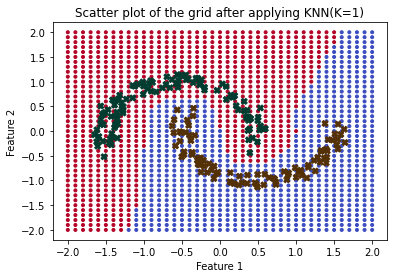
\includegraphics[width=8cm]{images/q2_1_grid.png}
        \caption{} \label{fig:q2_1}
	\end{figure}  
	\end{soln}
	
	
	\paragraph{Spam filter} Now, we will use 'emails.csv' as our dataset. The description is as follows.

	
	\begin{itemize}
		\item Task: spam detection
		\item The number of rows: 5000
		\item The number of features: 3000 (Word frequency in each email)
		\item The label (y) column name: `Predictor'
		\item For a single training/test set split, use Email 1-4000 as the training set, Email 4001-5000 as the test set.
		\item For 5-fold cross validation, split dataset in the following way.
		\begin{itemize}
			\item Fold 1, test set: Email 1-1000, training set: the rest (Email 1001-5000)
			\item Fold 2, test set: Email 1000-2000, training set: the rest
			\item Fold 3, test set: Email 2000-3000, training set: the rest
			\item Fold 4, test set: Email 3000-4000, training set: the rest
			\item Fold 5, test set: Email 4000-5000, training set: the rest			
		\end{itemize}
	\end{itemize}
	
	\item (8 pts) Implement 1NN, Run 5-fold cross validation. Report accuracy, precision, and recall in each fold.
	
	\begin{soln} The results of the implementation are as follows: \\
    \textbf{Fold:0}\\
    The precision score is:0.6544943820224719\\
    The recall score is:0.8175438596491228\\
    The accuracy score is:0.825\\
    \textbf{Fold:1}\\
    The precision score is:0.6857142857142857\\
    The recall score is:0.8664259927797834\\
    The accuracy score is:0.853\\
    \textbf{Fold:2}\\
    The precision score is:0.7212121212121212\\
    The recall score is:0.8380281690140845\\
    The accuracy score is:0.862\\
    \textbf{Fold:3}\\
    The precision score is:0.7164179104477612\\
    The recall score is:0.8163265306122449\\
    The accuracy score is:0.851\\
    \textbf{Fold:4}\\
    The precision score is:0.6057441253263708\\
    The recall score is:0.7581699346405228\\
    The accuracy score is:0.775 \\
    
    \end{soln}
	
	\item (12 pts) Implement logistic regression (from scratch). Use gradient descent (refer to question 6 from part 1) to find the optimal parameters. You may need to tune your learning rate to find a good optimum. Run 5-fold cross validation. Report accuracy, precision, and recall in each fold.
	
	\begin{soln} 
 I ran logistic regression for 1000 epochs with LR=5e-3 on all the folds. Using loss as criterion, I used the best model obtained for prediction. This was done without early stopping as it hasn't been covered yet in the class. One observation I could make is the fluctuating nature of the losses irrespective of the learning rate and the model learning even after 800-900 epochs. The results of the different folds are as follows:\\
    \textbf{Fold:0}\\
    The precision score is:0.8598484848484849\\
    The recall score is:0.7964912280701755\\
    The accuracy score is:0.905\\
    \textbf{Fold:1}\\
    The precision score is:0.8530612244897959\\
    The recall score is:0.7545126353790613\\
    The accuracy score is:0.896\\
    \textbf{Fold:2}\\
    The precision score is:0.5204081632653061\\
    The recall score is:0.897887323943662\\
    The accuracy score is:0.736\\
    \textbf{Fold:3}\\
    The precision score is:0.9591836734693877\\
    The recall score is:0.1598639455782313\\
    The accuracy score is:0.751\\
    \textbf{Fold:4}\\
    The precision score is:0.5380333951762524\\
    The recall score is:0.9477124183006536\\
    The accuracy score is:0.735\end{soln}
	
	\item (10 pts) Run 5-fold cross validation with kNN varying k (k=1, 3, 5, 7, 10). Plot the average accuracy versus k, and list the average accuracy of each case. \\
	Expected figure looks like this.
	
	
	\begin{soln} 
    The average accuracy for K=1 is: 0.8332.\\
    The average accuracy for K=3 is: 0.8422000000000001.\\
    The average accuracy for K=5 is: 0.8408.\\
    The average accuracy for K=7 is: 0.8462.\\
    The average accuracy for K=10 is: 0.8556000000000001.\\
    
    The accuracy plot is in Figure \ref{fig:q2_4}
    \begin{figure}[hbt!]
		\centering
		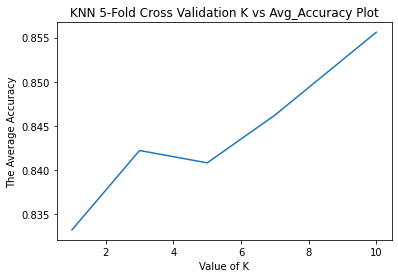
\includegraphics[width=8cm]{images/q2_4_K_vs_acc.png}
        \caption{} \label{fig:q2_4}
	\end{figure}
    \end{soln}
	
	\item (10 pts) Use a single training/test setting. Train kNN (k=5) and logistic regression on the training set, and draw ROC curves based on the test set. \\

	
	\begin{soln}
    The ROC curve for KNN (k=5) and Logistic Regression can be found in Figure \ref{fig:q2_5roc}.
    \begin{figure}[hbt!]
		\centering
		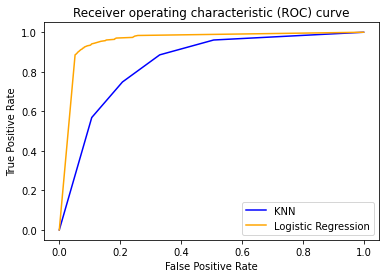
\includegraphics[width=8cm]{images/q2_5_roc.png}
        \caption{} \label{fig:q2_5roc}
	\end{figure} \end{soln}
	
\end{enumerate}
\bibliographystyle{apalike}
\end{document}
